
\documentclass[11pt,compress,t,notes=noshow, aspectratio=169, xcolor=table]{beamer}

\usepackage[nospeakermargin]{../../style/lmu-lecture-2}
% Defines macros and environments
% This file is included in slides and exercises

% Rarely used fontstyle for R packages, used only in 
% - forests/slides-forests-benchmark.tex
% - exercises/single-exercises/methods_l_1.Rnw
% - slides/cart/attic/slides_extra_trees.Rnw
\newcommand{\pkg}[1]{{\fontseries{b}\selectfont #1}}

% Spacing helpers, used often (mostly in exercises for \dlz)
\newcommand{\lz}{\vspace{0.5cm}} % vertical space (used often in slides)
\newcommand{\dlz}{\vspace{1cm}}  % double vertical space (used often in exercises, never in slides)
\newcommand{\oneliner}[1] % Oneliner for important statements, used e.g. in iml, algods
{\begin{block}{}\begin{center}\begin{Large}#1\end{Large}\end{center}\end{block}}

% Don't know if this is used or needed, remove?
% textcolor that works in mathmode
% https://tex.stackexchange.com/a/261480
% Used e.g. in forests/slides-forests-bagging.tex
% [...] \textcolor{blue}{\tfrac{1}{M}\sum^M_{m} [...]
% \makeatletter
% \renewcommand*{\@textcolor}[3]{%
%   \protect\leavevmode
%   \begingroup
%     \color#1{#2}#3%
%   \endgroup
% }
% \makeatother


\title{Applied Machine Learning}
% \author{LMU}
%\institute{\href{https://compstat-lmu.github.io/lecture_iml/}{compstat-lmu.github.io/lecture\_iml}}
\date{}

\begin{document}

\newcommand{\titlefigure}{figure/dtrain_dtest_resampling}
\newcommand{\learninggoals}{
\item What is the difference between a loss function and a performance metric?
\item What are desirable properties of a performance metric?
\item What are guiding questions to select a performance metric?}

\lecturechapter{Performance Metrics}
\lecture{Applied Machine Learning}


\begin{frame}{Considerations for Practice}

\begin{itemize}
    \item Stakeholders must grasp metrics relevant to the use case.
    \item What a model optimizes does not necessarily overlap with what we are trying to achieve in a specific use case.
    \item Choose performance metrics according to needs of the use case:
    \begin{itemize}
        \item Consider outlier sensitivity (e.g., MAE instead of MSE)
        \item Address class imbalance (e.g., F1 score instead of accuracy)
        %, PR-AUC vs. ROC-AUC)
        \item Cost-sensitive classification (e.g., use weights for FP/FN)
        \item Discrimination vs. calibration (predicting the correct class vs. interpreting predicted probabilities as actual risk) \newline
        $\Rightarrow$ Confusion matrix-based metrics vs. proper scoring rules
    \end{itemize}

\end{itemize}
\end{frame}

% \begin{frame}{Answering the Wrong Question}
% % A. W. Kimball (1957) Errors of the Third Kind in Statistical Consulting, Journal of the American Statistical Association, 52:278, 133-142
% \begin{itemize}
% \setlength\itemsep{1em}
%     \item An approximate answer to the right question is worth much more than the right answer to the wrong question.
%     \item Pay attention to but do not get lost in technical details. You might end up developing a model that answers the wrong question or optimizes the wrong metric.
%     \item \textbf{Example:} An online retail company aims to increase revenue by displaying advertisements with different products, hoping that the customer is going to purchase additional products. The company measures how often the user clicks / taps on those advertisements. A model is trained to predict click rates based on features such as the product category, price, age of the customer, etc. However, this model does not actually measure additional revenue from advertisements, as many customers will click on them by accident or not go through with the purchase.
% \end{itemize}
    
% \end{frame}

% \begin{frame}{What Affects Performance?}
% % https://vuquangnguyen2016.files.wordpress.com/2018/03/applied-predictive-modeling-max-kuhn-kjell-johnson_1518.pdf

% There is a multitude of technical aspects we need to consider:

% \begin{itemize}
%     \item \textbf{Model type:} Some models are or are not suited for certain tasks, e.g., tree-based models are bad at predicting linearly shaped data.
%     \item \textbf{Non-informative features:} Including features that are not correlated with the target increases the risk of modeling noise.
%     \item \textbf{Pre-processing of features:} Optimizing feature processing can improve performance, depending on the model.
%     %\item \textbf{Measurement errors / noise in the outcome or features:} Garbage in = garbage out. Our performance depends on the quality of model inputs.
%     \item \textbf{Data quality:} The presence of measurement errors or noise in both outcomes and features directly influences model efficacy (garbage in = garbage out).
%     \item \textbf{Sample size:} The more data we have at our disposal, the better our algorithm is able to learn from it.
%     %\item \textbf{Data diversity:} Beyond large sample size, diverse data also matters
% \end{itemize}
% \end{frame}




\begin{frame}{Loss Function vs. Performance Measure}

Both loss functions (LFs) and performance measures (PMs) serve to evaluate the performance of a model but for different purposes:

\begin{itemize}
    \item LFs are used to optimize model parameters \textbf{during training}. \\
    $\Rightarrow$ desirable numerical properties, e.g., differentiability
    \item PMs are used to evaluate the model performance \textbf{after training} on unseen test data. 
    \item PMs should be tailored to the task at hand, i.e., measure the model's ability to achieve the desired objective.
    %\item LFs shoud have desirable numerical properties, e.g., differentiability for gradient-based optimization, convexity, robustness against outliers, etc.
    \item Ideally, we set LF = PM but this is not always possible.\\
    $\Rightarrow$ LF is often specified by the ML algorithm, but we can tune its hyperparameters regarding our desired PM.
    % However, one typically selects the PM based on the prediction task and opts to approximate this metric with an LF that is numerically easier to handle.
    %\item LFs are often difficult to interpret. In contrast, a PM should be interpretable, as it is used to select an appropriate model from a number of candidates.
    %\item A PM should be tailored to the task at hand: what objective shall the model achieve and does the PM measure its ability to do so?
\end{itemize}
\end{frame}


\begin{frame}{Examples: LF versus PM}

\begin{itemize}
    \item \textbf{Regression:}
        \begin{itemize} 
            \item Models often optimize the mean squared error (MSE) during training (LF), which can also be used to evaluate various final model candidates (PM).
            \item Alternative PM: Different model candidates are also often compared using Pearson's coefficient of determination $R^2$ (or its adjusted variant) (PM).
        \end{itemize}
    \item \textbf{Classification:}
        \begin{itemize}
            \item The logarithmic loss is a popular LF to optimize classification models and can also be used as a PM.
            \item Alternative PM: The AUC (area under the ROC curve) compares the true positive rate against the false positive rate at each threshold setting.
        \end{itemize}
\end{itemize}    
\end{frame}

% \begin{frame}{Desirable Traits of a Performance Metrics}
%     \begin{itemize}
%         \item A PM should be tailored to the task at hand: what objective shall the model achieve and does the PM measure its ability to do so (on unseen data)?
%         \item A PM should be interpretable, as it is used to convey the model's ability to predict to various stakeholders.
%         \item It should be model-agnostic.
%     \end{itemize}
% \end{frame}


\begin{frame}{Selecting a Performance Measure: Task}

\begin{itemize}
    \item Selecting a performance measure is based on technical (task properties) and non-technical (stakeholder demands) requirements.
    \item We formulate specific guiding questions (GQs) addressing such requirements.
    \item The most fundamental GQ concerns the prediction task:
    \begin{figure}
        \centering
        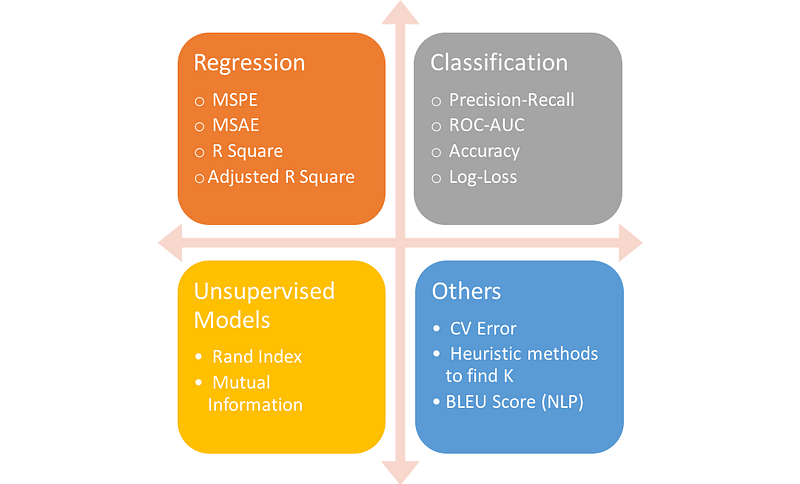
\includegraphics[width = 0.8\textwidth]{figure/metrics_task_overview.png}
    \end{figure}
\end{itemize}
    
\end{frame}


\begin{frame}{Overview for Classification}
    % https://www.kaggle.com/code/vipulgandhi/how-to-choose-right-metric-for-evaluating-ml-model
    % https://www.cambridge.org/core/books/evaluating-learning-algorithms/performance-measures-i/FED700405CB3E8FDE885528DF5D3060B
    % https://neptune.ai/blog/f1-score-accuracy-roc-auc-pr-auc
    \begin{figure}
        \centering
        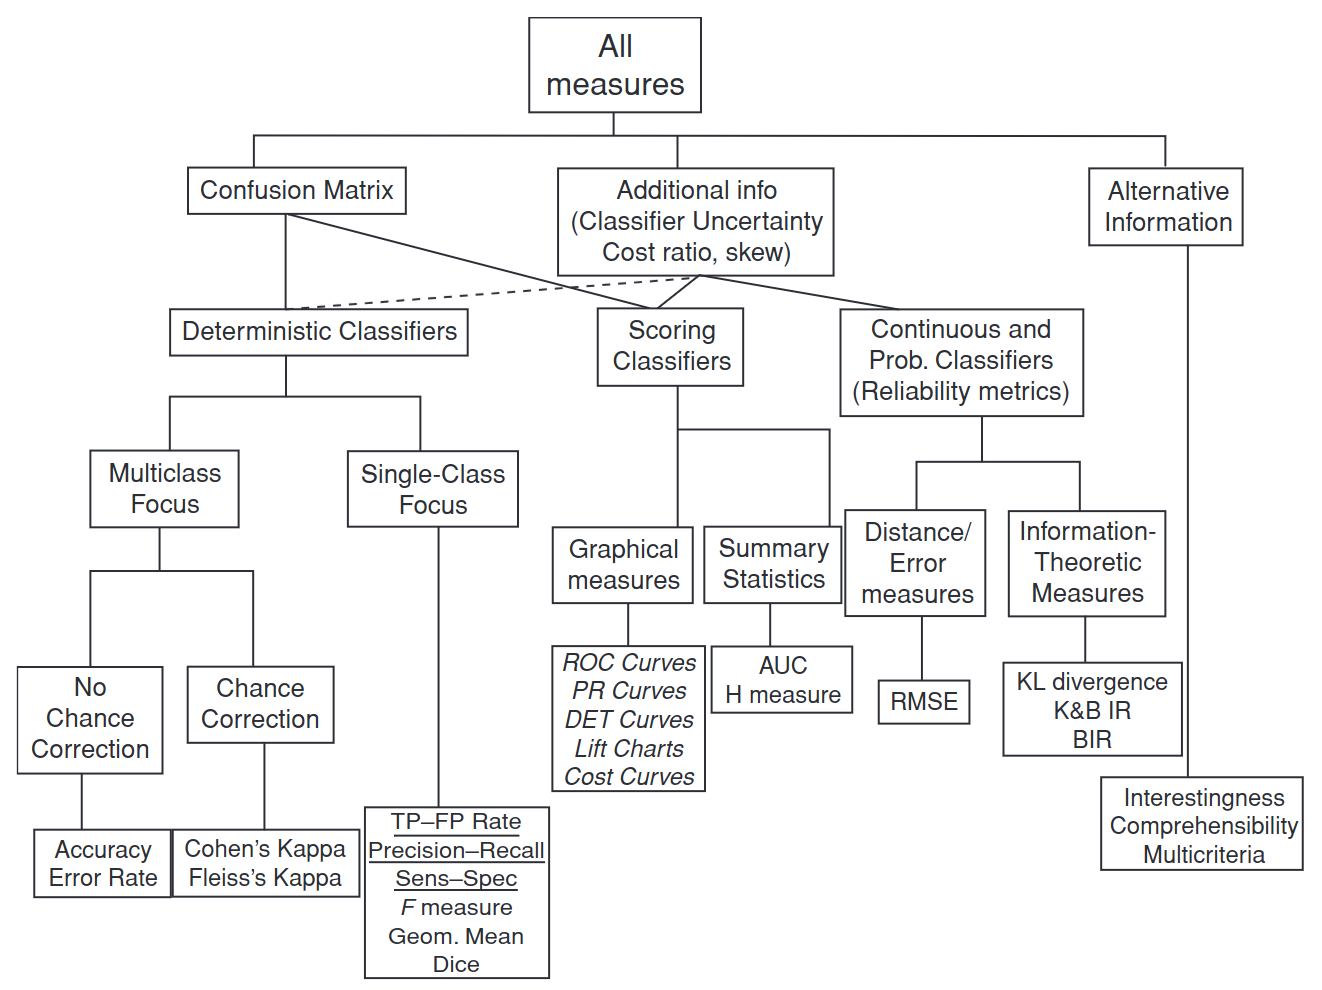
\includegraphics[width = 0.9\textwidth]{figure/classification_measures.png}
    \end{figure}
    
\end{frame}

\begin{frame}{GQ: Software Output?}
    \begin{itemize}
        \item Most software packages support both probability / score and hard label outputs.
        \item Probabilities / scores can always be converted to hard labels. However, in certain settings we may be stuck with hard label predictions.
        \item For hard labels, we are restricted to measures based on the confusion matrix: accuracy, error rate, precision, recall, null error rate, F score, Cohen's Kappa
        \item For soft labels, we can use additional measures as well including the ROC curve and AUC measure and the precision-recall curve.
    \end{itemize}
\end{frame}


\begin{frame}{GQ: Cost Sensitivity - True Positives?}
    \begin{itemize}
        \item For certain applications, identifying true positives and avoiding false negatives is more important than avoiding false positives (\enquote{a false alarm}). 
        \item For instance, when screening for cancer, missing to diagnose it will likely result in a fatal outcome for the patient, whereas a false positive may warrant additional investigations by doctors but no fatal outcome.
        \item Here, the true positive rate is important, which is also known as recall or sensitivity:
            $$
                \text{Sensitivity (recall or true positive rate)} = \frac{\text{\# true positives}}{\text{\# true positives + false negatives}}
            $$
    \end{itemize}
\end{frame}

% \begin{frame}{Guiding Question: Identifying True Positives?}
%     \begin{itemize}
%         \item
%         \setlength\itemsep{2em}
%         For certain applications, identifying true positives and avoiding false negatives is more important than avoiding false positives (\enquote{a false alarm}). 
%         \item For instance, when screening for cancer, missing to diagnose it will likely result in a fatal outcome for the patient, whereas a false positive may warrant additional investigations by doctors but no fatal outcome.
%         \item Here, the true positive rate is important, which is also known as recall or sensitivity:
%             $$
%                 \text{Recall (Sensitivity)} = \frac{\text{\# true positives}}{\text{\# true positives + false negatives}}
%             $$
%     \end{itemize}
% \end{frame}

\begin{frame}{GQ: Cost Sensitivity - True Negatives?}
    \begin{itemize}
        \item The reverse corresponds to focusing on the identification of true negatives and assigning a lesser cost to false positives.
        \item \textbf{Example:} In an automated underwriting, identifying all applicants who will not pay back the loan is more important than not lending to an applicant who would pay back the loan.
        \item Here, the true negative rate is an appropriate PM, which is also known as  specifity:
            $$
                \text{Specifity (true negative rate)} = \frac{\text{\# true negatives}}{\text{\# true negatives + false positives}}
            $$
    \end{itemize}
\end{frame}


\begin{frame}{GQ: Cost Sensitivity - Avoid False Positives?}
    \begin{itemize}
        \item In other applications, avoiding false positives may be most important.
        \item \textbf{Example:} For spam detection, we may not care about a few spam emails in our inbox folder (false negative), but we really want to avoid classifying an important email as spam (false positive).
        \item Here, maximizing precision, also known as the positive predictive value, is appropriate:
        $$
            \text{Precision (positive predictive value)} = \frac{\text{\# true positives}}{\text{\# true positives + false positives}}
        $$
    \end{itemize}
\end{frame}


\begin{frame}{GQ: Balanced Data}
    \begin{itemize}
        \item Accuracy is a good measure if roughly the same number of observations belong to each class (balanced data):
            $$
                \text{Accuracy} = \frac{\text{\# correct predictions}}{\text{\# total predictions}}
            $$
        \item \textbf{Example:} 
        \begin{itemize}
            \item Consider two classes A and B with 98\% of observations belonging to class A and 2\% to class B.
            \item A naive (and useless) model that always predicts class A will have 98\% accuracy and be falsely evaluated as a good model.
        \end{itemize}
        \item If we have imbalanced data, a good option is to use measures based on the confusion matrix such as precision, recall, the F1 score, or the Jaccard index.
        \item Unfortunately, there is no silver bullet for imbalanced data, and the selection of a suitable PM is still subject to ongoing research!
    \end{itemize}
\end{frame}

\begin{frame}{GQ: Imbalanced Data and Possible Options}
    \begin{itemize}
        \item One option is to modify the data to cure imbalances. Over- or undersampling copy instances from the minority and majority class to receive a balanced class distribution.
        \item A popular variant that does over- and undersampling simultaneously is called synthetic minority oversampling technique (SMOTE).
        \item SMOTE is highly controversial!
        \item But there are certain PMs that can be used in imbalanced settings as well.
    \end{itemize}
\end{frame}


% \begin{frame}{Guiding Question: Cost Sensitivity?}
%     % https://towardsdatascience.com/what-metrics-should-we-use-on-imbalanced-data-set-precision-recall-roc-e2e79252aeba
%     \begin{itemize}
%         \setlength\itemsep{1em}
%         \item Depending on which kind of imbalance we have and what we are trying to measure, different measures are preferable.
%         \item If our goal is to measure the ability to 
%         Precision is a good measure if the imbalance is towards the negative class:
%             $$
%                 \text{Accuracy} = \frac{\text{\# correct predictions}}{\text{\# total predictions}} \cdot 100
%             $$
%         \item If we have imbalanced data, a good option is to use metrics based on the confusion matrix such as precision, recall, the F1 score, or the Jaccard index.
%         \item \textbf{Example:} 
%             \vspace{0.5cm}
%         \begin{itemize}
%             \item Consider two classes A and B with 98\% of observations belonging to class A and 2\% to class B.
%             \item A naive (and useless) model that always predicts class A will have 98\% accuracy and be falsely evaluated as a good model.
%         \end{itemize}
%     \end{itemize}
% \end{frame}

% \begin{frame}{Cost Sensititivity - Identifying True Positives}
%     \begin{itemize}
%         \item
%         \setlength\itemsep{2em}
%         For certain applications, identifying true positives and avoiding false negatives is more important than predicting false positives (\enquote{a false alarm}). For instance, when screening for cancer, missing to diagnose it will likely result in a fatal outcome for the patient, whereas a false positive may warrant additional investigations by doctors but no fatal outcome.
%         \item Here, the true positive rate is important, which is also known as recall or sensitivity.
%     \end{itemize}
% \end{frame}

% \begin{frame}{Cost Sensititivity - Avoiding False Positives}
%     \begin{itemize}
%         \setlength\itemsep{2em}
%         \item In other applications, avoiding false positives may be most important.
%         \item \textbf{Example:} For spam detection, we may not care about a few spam emails in our inbox folder (false negative), but we really want to avoid classifying an important email as spam (false positive).
%         \item Here, precision is the right measure.
%     \end{itemize}
% \end{frame}

% \begin{frame}{Cost Sensitivity - Identifying True Negatives}
%     \begin{itemize}
%         \setlength\itemsep{2em}
%         \item Lastly, we may want to identify all true negatives and accept some false positives.
%         \item An example could be an automated credit loan decision. Identifying all applicants with bad credit ratings (i.e., who will not pay back the loan) is more important than not giving a loan to an applicant with a good credit rating (who would pay back the loan).
%     \end{itemize}
% \end{frame}


% \begin{frame}{Output of Classification Software}
    
% \end{frame}

% \begin{frame}{Selecting an Established Metric}

% \begin{figure}
%     \centering
%     \includegraphics[width = 0.85\textwidth]{figure/ontology_perf_metrics.png}
% \end{figure}
% \end{frame}

% \begin{frame}{Selecting an Established Metric}

% \begin{figure}
%     \centering
%     \includegraphics[width = 0.85\textwidth]{figure/classification_of_metrics.png}
% \end{figure}
% \end{frame}

% xx
% % \begin{frame}{Established Performance Metrics}

% % \begin{itemize}
% % \setlength\itemsep{2em}
% %     \item List and motivate established performance metrics here
% %     \item E.g., for \textbf{classification}: accuracy, true and false positive rate, precision and recall, F-score, AUC, Brier score
% %     \item E.g., for \textbf{regression}: MSE, RMSE, MAE, R2
% %     \item Describe typical use case and why metric works
% %     \item Example: Brier Score rewards model confidence (i.e. give a high probability to a true outcome) and punishes the reverse.
% % \end{itemize}
% % \end{frame}

\begin{frame}{Advanced Performance Metrics}

\begin{itemize}
    \item Dive into esoteric stuff here: Youden, Cohens-Kappa, Matthews correlation
    \item Motivate each advanced metric, do not just list formula
    \item Example: "MCC produces a high score only if the prediction obtained good results in all of the confusion matrix categories (TP, FP, TN, FN), proportionally both to the size of positive elements and the size of negative elements in the dataset"
\end{itemize}
\end{frame}



\endlecture
\end{document}
